% Created by tikzDevice version 0.12.6 on 2024-03-17 14:52:39
% !TEX encoding = UTF-8 Unicode
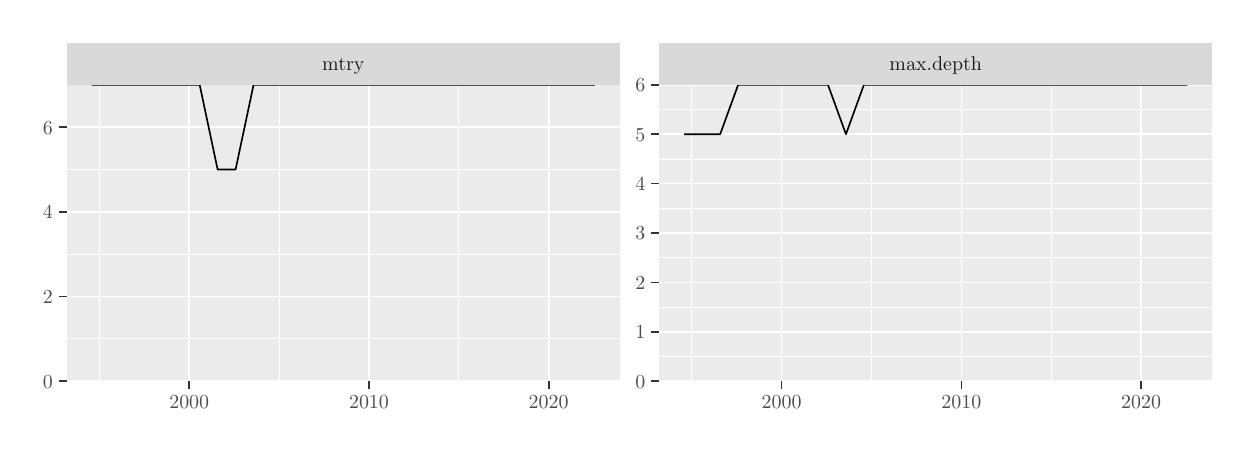
\begin{tikzpicture}[x=1pt,y=1pt]
\definecolor{fillColor}{RGB}{255,255,255}
\path[use as bounding box,fill=fillColor,fill opacity=0.00] (0,0) rectangle (433.62,144.54);
\begin{scope}
\path[clip] (  0.00,  0.00) rectangle (433.62,144.54);
\definecolor{drawColor}{RGB}{255,255,255}
\definecolor{fillColor}{RGB}{255,255,255}

\path[draw=drawColor,line width= 0.6pt,line join=round,line cap=round,fill=fillColor] (  0.00,  0.00) rectangle (433.62,144.54);
\end{scope}
\begin{scope}
\path[clip] ( 14.05, 16.81) rectangle (214.06,123.88);
\definecolor{fillColor}{gray}{0.92}

\path[fill=fillColor] ( 14.05, 16.81) rectangle (214.06,123.88);
\definecolor{drawColor}{RGB}{255,255,255}

\path[draw=drawColor,line width= 0.3pt,line join=round] ( 14.05, 32.10) --
	(214.06, 32.10);

\path[draw=drawColor,line width= 0.3pt,line join=round] ( 14.05, 62.70) --
	(214.06, 62.70);

\path[draw=drawColor,line width= 0.3pt,line join=round] ( 14.05, 93.29) --
	(214.06, 93.29);

\path[draw=drawColor,line width= 0.3pt,line join=round] ( 14.05,123.88) --
	(214.06,123.88);

\path[draw=drawColor,line width= 0.3pt,line join=round] ( 25.91, 16.81) --
	( 25.91,123.88);

\path[draw=drawColor,line width= 0.3pt,line join=round] ( 90.85, 16.81) --
	( 90.85,123.88);

\path[draw=drawColor,line width= 0.3pt,line join=round] (155.79, 16.81) --
	(155.79,123.88);

\path[draw=drawColor,line width= 0.6pt,line join=round] ( 14.05, 16.81) --
	(214.06, 16.81);

\path[draw=drawColor,line width= 0.6pt,line join=round] ( 14.05, 47.40) --
	(214.06, 47.40);

\path[draw=drawColor,line width= 0.6pt,line join=round] ( 14.05, 77.99) --
	(214.06, 77.99);

\path[draw=drawColor,line width= 0.6pt,line join=round] ( 14.05,108.59) --
	(214.06,108.59);

\path[draw=drawColor,line width= 0.6pt,line join=round] ( 58.38, 16.81) --
	( 58.38,123.88);

\path[draw=drawColor,line width= 0.6pt,line join=round] (123.33, 16.81) --
	(123.33,123.88);

\path[draw=drawColor,line width= 0.6pt,line join=round] (188.26, 16.81) --
	(188.26,123.88);
\definecolor{drawColor}{RGB}{0,0,0}

\path[draw=drawColor,line width= 0.6pt,line join=round] ( 23.14,123.88) --
	( 29.67,123.88) --
	( 36.17,123.88) --
	( 42.66,123.88) --
	( 49.15,123.88) --
	( 55.62,123.88) --
	( 62.15,123.88) --
	( 68.64, 93.29) --
	( 75.13, 93.29) --
	( 81.62,123.88) --
	( 88.11,123.88) --
	( 94.58,123.88) --
	(101.10,123.88) --
	(107.59,123.88) --
	(114.10,123.88) --
	(120.59,123.88) --
	(127.06,123.88) --
	(133.53,123.88) --
	(140.07,123.88) --
	(146.56,123.88) --
	(153.05,123.88) --
	(159.54,123.88) --
	(166.01,123.88) --
	(172.54,123.88) --
	(179.03,123.88) --
	(185.52,123.88) --
	(192.03,123.88) --
	(198.50,123.88) --
	(204.97,123.88);
\end{scope}
\begin{scope}
\path[clip] (228.11, 16.81) rectangle (428.12,123.88);
\definecolor{fillColor}{gray}{0.92}

\path[fill=fillColor] (228.11, 16.81) rectangle (428.12,123.88);
\definecolor{drawColor}{RGB}{255,255,255}

\path[draw=drawColor,line width= 0.3pt,line join=round] (228.11, 25.73) --
	(428.12, 25.73);

\path[draw=drawColor,line width= 0.3pt,line join=round] (228.11, 43.58) --
	(428.12, 43.58);

\path[draw=drawColor,line width= 0.3pt,line join=round] (228.11, 61.42) --
	(428.12, 61.42);

\path[draw=drawColor,line width= 0.3pt,line join=round] (228.11, 79.27) --
	(428.12, 79.27);

\path[draw=drawColor,line width= 0.3pt,line join=round] (228.11, 97.11) --
	(428.12, 97.11);

\path[draw=drawColor,line width= 0.3pt,line join=round] (228.11,114.96) --
	(428.12,114.96);

\path[draw=drawColor,line width= 0.3pt,line join=round] (239.97, 16.81) --
	(239.97,123.88);

\path[draw=drawColor,line width= 0.3pt,line join=round] (304.91, 16.81) --
	(304.91,123.88);

\path[draw=drawColor,line width= 0.3pt,line join=round] (369.85, 16.81) --
	(369.85,123.88);

\path[draw=drawColor,line width= 0.6pt,line join=round] (228.11, 16.81) --
	(428.12, 16.81);

\path[draw=drawColor,line width= 0.6pt,line join=round] (228.11, 34.65) --
	(428.12, 34.65);

\path[draw=drawColor,line width= 0.6pt,line join=round] (228.11, 52.50) --
	(428.12, 52.50);

\path[draw=drawColor,line width= 0.6pt,line join=round] (228.11, 70.34) --
	(428.12, 70.34);

\path[draw=drawColor,line width= 0.6pt,line join=round] (228.11, 88.19) --
	(428.12, 88.19);

\path[draw=drawColor,line width= 0.6pt,line join=round] (228.11,106.04) --
	(428.12,106.04);

\path[draw=drawColor,line width= 0.6pt,line join=round] (228.11,123.88) --
	(428.12,123.88);

\path[draw=drawColor,line width= 0.6pt,line join=round] (272.44, 16.81) --
	(272.44,123.88);

\path[draw=drawColor,line width= 0.6pt,line join=round] (337.39, 16.81) --
	(337.39,123.88);

\path[draw=drawColor,line width= 0.6pt,line join=round] (402.32, 16.81) --
	(402.32,123.88);
\definecolor{drawColor}{RGB}{0,0,0}

\path[draw=drawColor,line width= 0.6pt,line join=round] (237.20,106.04) --
	(243.73,106.04) --
	(250.23,106.04) --
	(256.72,123.88) --
	(263.21,123.88) --
	(269.68,123.88) --
	(276.21,123.88) --
	(282.70,123.88) --
	(289.19,123.88) --
	(295.68,106.04) --
	(302.17,123.88) --
	(308.64,123.88) --
	(315.16,123.88) --
	(321.65,123.88) --
	(328.16,123.88) --
	(334.65,123.88) --
	(341.12,123.88) --
	(347.59,123.88) --
	(354.13,123.88) --
	(360.62,123.88) --
	(367.11,123.88) --
	(373.60,123.88) --
	(380.07,123.88) --
	(386.60,123.88) --
	(393.09,123.88) --
	(399.58,123.88) --
	(406.09,123.88) --
	(412.56,123.88) --
	(419.03,123.88);
\end{scope}
\begin{scope}
\path[clip] ( 14.05,123.88) rectangle (214.06,139.04);
\definecolor{fillColor}{gray}{0.85}

\path[fill=fillColor] ( 14.05,123.88) rectangle (214.06,139.04);
\definecolor{drawColor}{gray}{0.10}

\node[text=drawColor,anchor=base,inner sep=0pt, outer sep=0pt, scale=  0.72] at (114.05,128.98) {mtry};
\end{scope}
\begin{scope}
\path[clip] (228.11,123.88) rectangle (428.12,139.04);
\definecolor{fillColor}{gray}{0.85}

\path[fill=fillColor] (228.11,123.88) rectangle (428.12,139.04);
\definecolor{drawColor}{gray}{0.10}

\node[text=drawColor,anchor=base,inner sep=0pt, outer sep=0pt, scale=  0.72] at (328.11,128.98) {max.depth};
\end{scope}
\begin{scope}
\path[clip] (  0.00,  0.00) rectangle (433.62,144.54);
\definecolor{drawColor}{gray}{0.20}

\path[draw=drawColor,line width= 0.6pt,line join=round] ( 58.38, 14.06) --
	( 58.38, 16.81);

\path[draw=drawColor,line width= 0.6pt,line join=round] (123.33, 14.06) --
	(123.33, 16.81);

\path[draw=drawColor,line width= 0.6pt,line join=round] (188.26, 14.06) --
	(188.26, 16.81);
\end{scope}
\begin{scope}
\path[clip] (  0.00,  0.00) rectangle (433.62,144.54);
\definecolor{drawColor}{gray}{0.30}

\node[text=drawColor,anchor=base,inner sep=0pt, outer sep=0pt, scale=  0.72] at ( 58.38,  6.90) {2000};

\node[text=drawColor,anchor=base,inner sep=0pt, outer sep=0pt, scale=  0.72] at (123.33,  6.90) {2010};

\node[text=drawColor,anchor=base,inner sep=0pt, outer sep=0pt, scale=  0.72] at (188.26,  6.90) {2020};
\end{scope}
\begin{scope}
\path[clip] (  0.00,  0.00) rectangle (433.62,144.54);
\definecolor{drawColor}{gray}{0.20}

\path[draw=drawColor,line width= 0.6pt,line join=round] (272.44, 14.06) --
	(272.44, 16.81);

\path[draw=drawColor,line width= 0.6pt,line join=round] (337.39, 14.06) --
	(337.39, 16.81);

\path[draw=drawColor,line width= 0.6pt,line join=round] (402.32, 14.06) --
	(402.32, 16.81);
\end{scope}
\begin{scope}
\path[clip] (  0.00,  0.00) rectangle (433.62,144.54);
\definecolor{drawColor}{gray}{0.30}

\node[text=drawColor,anchor=base,inner sep=0pt, outer sep=0pt, scale=  0.72] at (272.44,  6.90) {2000};

\node[text=drawColor,anchor=base,inner sep=0pt, outer sep=0pt, scale=  0.72] at (337.39,  6.90) {2010};

\node[text=drawColor,anchor=base,inner sep=0pt, outer sep=0pt, scale=  0.72] at (402.32,  6.90) {2020};
\end{scope}
\begin{scope}
\path[clip] (  0.00,  0.00) rectangle (433.62,144.54);
\definecolor{drawColor}{gray}{0.30}

\node[text=drawColor,anchor=base east,inner sep=0pt, outer sep=0pt, scale=  0.72] at (223.16, 14.33) {0};

\node[text=drawColor,anchor=base east,inner sep=0pt, outer sep=0pt, scale=  0.72] at (223.16, 32.17) {1};

\node[text=drawColor,anchor=base east,inner sep=0pt, outer sep=0pt, scale=  0.72] at (223.16, 50.02) {2};

\node[text=drawColor,anchor=base east,inner sep=0pt, outer sep=0pt, scale=  0.72] at (223.16, 67.87) {3};

\node[text=drawColor,anchor=base east,inner sep=0pt, outer sep=0pt, scale=  0.72] at (223.16, 85.71) {4};

\node[text=drawColor,anchor=base east,inner sep=0pt, outer sep=0pt, scale=  0.72] at (223.16,103.56) {5};

\node[text=drawColor,anchor=base east,inner sep=0pt, outer sep=0pt, scale=  0.72] at (223.16,121.40) {6};
\end{scope}
\begin{scope}
\path[clip] (  0.00,  0.00) rectangle (433.62,144.54);
\definecolor{drawColor}{gray}{0.20}

\path[draw=drawColor,line width= 0.6pt,line join=round] (225.36, 16.81) --
	(228.11, 16.81);

\path[draw=drawColor,line width= 0.6pt,line join=round] (225.36, 34.65) --
	(228.11, 34.65);

\path[draw=drawColor,line width= 0.6pt,line join=round] (225.36, 52.50) --
	(228.11, 52.50);

\path[draw=drawColor,line width= 0.6pt,line join=round] (225.36, 70.34) --
	(228.11, 70.34);

\path[draw=drawColor,line width= 0.6pt,line join=round] (225.36, 88.19) --
	(228.11, 88.19);

\path[draw=drawColor,line width= 0.6pt,line join=round] (225.36,106.04) --
	(228.11,106.04);

\path[draw=drawColor,line width= 0.6pt,line join=round] (225.36,123.88) --
	(228.11,123.88);
\end{scope}
\begin{scope}
\path[clip] (  0.00,  0.00) rectangle (433.62,144.54);
\definecolor{drawColor}{gray}{0.30}

\node[text=drawColor,anchor=base east,inner sep=0pt, outer sep=0pt, scale=  0.72] at (  9.10, 14.33) {0};

\node[text=drawColor,anchor=base east,inner sep=0pt, outer sep=0pt, scale=  0.72] at (  9.10, 44.92) {2};

\node[text=drawColor,anchor=base east,inner sep=0pt, outer sep=0pt, scale=  0.72] at (  9.10, 75.51) {4};

\node[text=drawColor,anchor=base east,inner sep=0pt, outer sep=0pt, scale=  0.72] at (  9.10,106.11) {6};
\end{scope}
\begin{scope}
\path[clip] (  0.00,  0.00) rectangle (433.62,144.54);
\definecolor{drawColor}{gray}{0.20}

\path[draw=drawColor,line width= 0.6pt,line join=round] ( 11.30, 16.81) --
	( 14.05, 16.81);

\path[draw=drawColor,line width= 0.6pt,line join=round] ( 11.30, 47.40) --
	( 14.05, 47.40);

\path[draw=drawColor,line width= 0.6pt,line join=round] ( 11.30, 77.99) --
	( 14.05, 77.99);

\path[draw=drawColor,line width= 0.6pt,line join=round] ( 11.30,108.59) --
	( 14.05,108.59);
\end{scope}
\end{tikzpicture}
